% =====================================================================
% Paper 15 - Fusing Real-Time and Scheduled Endpoint Telemetry for
% Vulnerability Visibility. IEEE TNSM submission. Build with tectonic.
% Reproducibility: results/primary_v1/ (125 rows = 25 seeds x 5 overlap
% levels; frozen on seeds 1000-1024). Run src/run_evaluation.py.
% =====================================================================
\documentclass[journal]{IEEEtran}

\usepackage{graphicx}
\usepackage{booktabs}
\usepackage{amsmath}
\usepackage{amssymb}
\usepackage{newtxtext,newtxmath}
\usepackage{hyperref}
\usepackage{xurl}
\usepackage{url}
\usepackage{array}

\graphicspath{{figures/}}

\title{Fusing Real-Time and Scheduled Endpoint Telemetry for Vulnerability\\
Visibility: Coverage Gains, the Freshness Mechanism, and the Blind-Spot Floor}

\author{%
  \IEEEauthorblockN{Harshavardhan Malla}
  \IEEEauthorblockA{Independent Researcher\\ Email: harshavardhanmalla75@gmail.com}%
}

\renewcommand{\textendash}{-}
\renewcommand{\textemdash}{-}
\usepackage{etoolbox}
\makeatletter
\patchcmd{\abstract}{---}{:\space}{}{}
\patchcmd{\IEEEkeywords}{---}{:\space}{}{}
\makeatother
\begin{document}
\maketitle

\begin{abstract}
State agency cyber-operations teams routinely run two endpoint-management tools with different
strengths: a real-time agent that reports fresh state for the assets it covers, and a scheduled
platform that covers a different, overlapping set but reports on a scan cadence and is often stale.
Building a current vulnerability heatmap of the fleet means fusing these partial, differently-fresh
feeds, yet the magnitude of the benefit and its limits are not obvious. We quantify both with a
pre-registered simulation of a 5{,}000-asset fleet, with hypotheses, thresholds, and evaluation
seeds locked before any result was inspected. At the reference coverage overlap, fusion detects
current vulnerabilities at recall 0.8702 against 0.7498 for the better single tool, a gain of
0.1204 (95\% bias-corrected and accelerated bootstrap interval $[0.1173, 0.1232]$), which clears
the pre-registered 0.10 bar. The gain has an exact mechanism: it equals the fresh coverage unique
to the scheduled feed, because the real-time feed already supplies full freshness on its own
coverage (difference 0.0, $[-0.0, 0.0]$). The benefit is bounded by a blind-spot floor of 0.051 of
the assets, those covered by neither tool, so the fusion miss of 0.1298 cannot fall below it. Across the
overlap sweep the gain falls monotonically from 0.1489 to 0.0 as the tools' coverage becomes
redundant, while the blind spot grows from 0.0 to 0.2475, so high overlap is doubly unfavorable.
The deployment rule is to fuse complementary, low-overlap tools and to treat the blind spot, not
the fusion logic, as the binding constraint on visibility. A closed-form analysis derives each of
these results exactly from the feeds' coverage and freshness, showing the gain to equal the
scheduled-only-fresh coverage and the blind spot to be a hard floor that an adversary can exploit by
placing assets where neither feed reaches.
\end{abstract}

\begin{IEEEkeywords}
asset visibility, data fusion, endpoint telemetry, vulnerability management, coverage, staleness,
blind spots, pre-registration, reproducibility
\end{IEEEkeywords}

\section{Introduction}
\IEEEPARstart{A}{n} authorizing official can only manage the risk that the inventory makes visible.
Federal asset-visibility guidance directs agencies to maintain a current account of the endpoints
on their networks and of the vulnerabilities those endpoints carry~\cite{cisabod2301,nist80137},
and the continuous-monitoring program that supports it treats visibility as an ongoing obligation
rather than a periodic snapshot~\cite{nist80137a}. The practical difficulty is that no single tool
delivers this current account. A real-time endpoint agent reports fresh state for the assets it has
been deployed to, but it never reaches the whole fleet: unmanaged hosts, network appliances, and
machines outside its install base fall outside its view. A scheduled management platform covers a
different and only partly overlapping set of assets, but it reports on a scan cadence, so the state
it shows is as old as the last scan and is frequently stale relative to the rate at which
vulnerabilities appear and are patched.

Cyber-operations teams resolve this by fusing the two feeds into one heatmap. Multisensor data
fusion is the established discipline for exactly this situation: combining complementary sources of
different quality, coverage, and timeliness into a single estimate that is better than any source
alone~\cite{hall1997fusion}, a practice that intrusion-detection research carried into security
operations decades ago~\cite{bass2000fusion}. The intuition that fusing a fresh-but-partial feed
with a broad-but-stale feed should help is sound, but it is only an intuition. How much does fusion
actually improve current-vulnerability visibility over the better single tool? What is the
mechanism, so that a team can predict the gain from the properties of its two tools rather than
discovering it after deployment? And what bounds the benefit, so that a program does not promise
visibility that fusion structurally cannot deliver?

This paper answers those three questions with a transparent model and a pre-registered evaluation.
We do not claim to measure any particular agency's posture; we build an explicit model of two feeds
with documented coverage and freshness probabilities, lock a set of hypotheses and thresholds in a
dated protocol before inspecting any evaluation seed, and report what the model says with
bias-corrected and accelerated bootstrap intervals~\cite{efron1987bca} rather than
significance tests. The contribution is fourfold.

\begin{itemize}
\item We \emph{quantify the fusion gain}. At the reference coverage overlap, fusing the two feeds
raises detection recall from 0.7498 for the better single tool to 0.8702, a gain of 0.1204
($[0.1173, 0.1232]$) that clears a pre-registered 0.10 bar.
\item We \emph{identify the exact mechanism}. The fusion gain over the real-time feed equals,
to the resolution of the experiment, the fresh coverage that only the scheduled feed adds
(difference 0.0, $[-0.0, 0.0]$), because the real-time feed already supplies full freshness on its
own coverage. The gain is therefore predictable from the scheduled feed's unique fresh reach.
\item We \emph{establish a blind-spot floor}. Assets that neither tool covers place a hard lower
bound on missed vulnerabilities. The fusion miss of 0.1298 exceeds this floor of 0.051
($[0.0489, 0.0539]$), and no fusion logic can detect below it; only new coverage can.
\item We \emph{characterize the overlap dependence}. The gain decreases monotonically as the two
tools' coverage overlaps and becomes redundant, from 0.1489 at low overlap to 0.0 at full overlap,
while the blind spot simultaneously grows from 0.0 to 0.2475, so high overlap is doubly
unfavorable.
\end{itemize}

The methodology is deliberately conservative. Every quantitative claim is a pre-registered
hypothesis evaluated on seeds that were not inspected during model development, and every interval
is a BCa bootstrap interval~\cite{efron1987bca,efron1994introduction} rather than a
null-hypothesis significance test, following the pre-registration discipline now standard in
empirical software engineering~\cite{wohlin2012experimentation}.

\section{Background and Related Work}

\subsection{Multisensor and data fusion}
The combination of complementary sensors into a single, better estimate is the founding idea of
multisensor data fusion~\cite{hall1997fusion}. The discipline distinguishes sources by their
coverage, accuracy, and timeliness, and provides a vocabulary for the levels at which they can be
combined, from raw-signal alignment to decision-level voting. Security operations adopted these
ideas early: fusing the alerts of multiple intrusion-detection sensors was proposed as a way to
raise true-positive coverage while suppressing the noise of any single sensor~\cite{bass2000fusion}.
Our setting is a decision-level fusion of two detection feeds, where the relevant axes are coverage
(which assets a feed can see) and freshness (whether what it reports is current). We make those two
axes explicit and derive the gain from them, rather than treating fusion as an opaque combiner.

\subsection{Anomaly and vulnerability detection}
Detection in security operations has a long lineage in anomaly detection, whose surveys catalog the
recurring trade-off between catching more events and tolerating more noise~\cite{chandola2009anomaly}.
A vulnerability heatmap is a detection problem of this kind: each asset either does or does not
carry a current vulnerability, and a feed either does or does not report it. Because the cost of a
missed current vulnerability dominates, recall is the operationally meaningful metric, and the
precision-recall framing is the appropriate evaluation lens for the skewed, miss-sensitive regime
we study~\cite{davis2006pr}. Our reproducible cyber-hygiene benchmark, together with prior
prioritization work in this program, established that endpoint telemetry arrives over several
distinct channels with different reliability and
timeliness~\cite{paper4hygieneprio,paper1vulnprio}; the present paper isolates the
coverage-and-freshness structure of two such channels and the consequences of fusing them.

\subsection{Federal asset-visibility mandates}
The motivation is not abstract. The federal binding operational directive on asset visibility
requires agencies to discover their assets and detect vulnerabilities on a regular cadence across
the whole fleet~\cite{cisabod2301}, and the continuous-monitoring framework that surrounds
it~\cite{nist80137,nist80137a} reframes visibility as an ongoing program. The control
catalog~\cite{nist80053} and the categorization standard~\cite{fips199} that determine which assets
matter most assume an inventory that is both broad and current, which is precisely what a single
tool cannot supply and fusion is meant to approximate. Breach data continues to attribute incidents
to known, unremediated weaknesses~\cite{verizon2026dbir}, so the assets a visibility program misses
are not an academic concern; they are where exposure concentrates. The autonomic-computing vision of
systems that continuously sense and manage their own state~\cite{kephart2003vision} anticipated this
shift toward fused, continuous self-assessment.

\subsection{Evaluation discipline}
We follow the evaluation conventions of empirical software engineering~\cite{wohlin2012experimentation}:
hypotheses and thresholds are fixed before the evaluation data are seen, and uncertainty is reported
as a bootstrap interval. We use the bias-corrected and accelerated bootstrap~\cite{efron1987bca,efron1994introduction}
because the statistics of interest are small-sample and possibly skewed, and we judge claims by
interval non-overlap rather than by significance tests, avoiding the multiple-comparison hazards of
repeated $p$-values across four hypotheses and five overlap levels.

\section{System Model}
\label{sec:model}
We model a fleet of endpoints observed by two feeds and ask how much current-vulnerability
visibility each monitoring regime delivers. All quantities are synthetic with documented
distributions; no operational, employer, or telemetry data is used.

\subsection{Fleet and coverage}
Each seed instantiates a fleet of $N = 5{,}000$ assets. The real-time feed $R$ covers each asset
with marginal probability $c_R = 0.75$; the scheduled feed $S$ covers each asset with marginal
probability $c_S = 0.70$. The joint coverage is parameterized by the probability $p_{\cap}$ that an
asset is covered by both feeds, which we sweep over $\{0.45, 0.50, 0.55, 0.60, 0.70\}$ with $0.50$
as the reference. Each asset thus falls into one of four coverage classes: both feeds, real-time
only, scheduled only, or neither. The four class probabilities follow directly from the marginals
and $p_{\cap}$,
\begin{equation}
\Pr(R\text{ only}) = c_R - p_{\cap}, \quad \Pr(S\text{ only}) = c_S - p_{\cap},
\label{eq:classes}
\end{equation}
and the \emph{blind-spot rate}, the share of assets that neither feed covers, is the complement of
the coverage union,
\begin{equation}
\beta \;=\; 1 - \big(c_R + c_S - p_{\cap}\big)\;=\; 1 - c_R - c_S + p_{\cap}.
\label{eq:blindspot}
\end{equation}
The blind-spot rate rises one-for-one with the overlap $p_{\cap}$: the more the two feeds duplicate
each other's coverage, the less of the fleet they jointly reach. At the reference overlap this gives
$\beta = 0.051$, and across the sweep it grows from 0.0 to 0.2475.

\subsection{Freshness and detection}
Each asset carries a true current vulnerability with prevalence $0.30$; this only sizes the
evaluated sample, since recall is computed over the current-vulnerability assets. A feed
\emph{detects} a current vulnerability when it covers the asset and its report is fresh. The
real-time feed is fresh wherever it covers, reflecting its continuous reporting. The scheduled feed
is fresh with probability $\phi = 0.60$ where it covers, the remaining $0.40$ being stale because
the scan cadence is slower than the rate at which vulnerabilities change. The per-feed recalls are
therefore approximately constant across overlap levels, governed by coverage and freshness rather
than by how the two feeds relate: the real-time feed detects at recall about $0.75$ and the
scheduled feed at recall about $0.42$, the latter being its coverage discounted by its freshness.

\subsection{The fusion rule and its gain}
Fusion takes the freshest available signal per asset: a current vulnerability is detected if the
real-time feed covers the asset, or the scheduled feed covers it and is fresh. This is a
decision-level union of detections,
\begin{equation}
\mathrm{Detect}_{\text{fuse}} \;=\; \big[\,R\text{ covers}\,\big] \;\vee\; \big[\,S\text{ covers} \;\wedge\; S\text{ fresh}\,\big].
\label{eq:fusion}
\end{equation}
Because the real-time feed already contributes full freshness on everything it covers, fusion adds
exactly the assets the real-time feed does \emph{not} cover but the scheduled feed does and reports
fresh. That increment, the \emph{scheduled-only-fresh coverage} $\phi\,(c_S - p_{\cap})$, is the
entire source of the fusion gain over the real-time feed. Detection recall is the fraction of
current-vulnerability assets a regime detects~\cite{davis2006pr}; the fusion miss rate is one minus
fusion recall, and it can never fall below the blind-spot rate $\beta$ of Eq.~(\ref{eq:blindspot}),
because an asset neither feed covers cannot be detected by any combination rule. The blind spot is
thus a floor on misses that fusion is structurally unable to lower; only extending coverage can.

\section{Theoretical Analysis}
\label{sec:theory}
The three empirical findings are not coincidences of the chosen constants; each follows in closed
form from the coverage-and-freshness structure of Section~\ref{sec:model}. This section derives the
fusion identity exactly, shows that the fusion gain over the better single feed equals the
scheduled-only-fresh coverage with no residual, proves the blind-spot floor on misses, and
characterizes how the gain decays as the feeds become redundant. We then check each derived value
against the frozen results and state the match explicitly.

Throughout we work over the population of current-vulnerability assets, since recall is computed on
that population (Section~\ref{sec:model}). Detection by a feed is a coverage-and-freshness event.
Let an asset be covered by the real-time feed $R$ with marginal probability $c_R$ and by the
scheduled feed $S$ with marginal probability $c_S$, with both-feed probability $p_{\cap}$. Write
$\phi$ for the scheduled feed's freshness, and recall that the real-time feed is fresh wherever it
covers. With $r_{\mathrm{rt}}$ the probability that the real-time feed detects an asset's current
vulnerability, the model's freshness assumption gives the per-feed recalls in closed form,
\begin{equation}
r_{\mathrm{rt}} \;=\; c_R, \qquad r_{\mathrm{sch}} \;=\; \phi\,c_S,
\label{eq:single_recalls}
\end{equation}
because the real-time feed detects exactly where it covers, while the scheduled feed detects only
where it both covers and is fresh.

\subsection{The fusion identity in closed form}
Fusion detects a current vulnerability when the real-time feed covers the asset, or the scheduled
feed covers it and is fresh (Eq.~\ref{eq:fusion}). Equivalently, fusion misses an asset only when
\emph{neither} feed detects it: the real-time feed does not cover it, and the scheduled feed either
does not cover it or covers it stale. Writing the fused recall as one minus the probability that
neither feed detects,
\begin{equation}
\mathrm{recall}_{\text{fuse}}
\;=\; 1 - \Pr\!\big(R\text{ misses}\,\wedge\, S\text{ misses fresh}\big).
\label{eq:fuse_complement}
\end{equation}
The real-time feed misses with probability $1 - c_R$ (its uncovered assets), and these are exactly
the assets where the scheduled feed must carry the load. Conditioning on the real-time miss and
using the coverage accounting of Eq.~(\ref{eq:classes}), the scheduled feed covers a real-time-miss
asset and reports it fresh precisely on the scheduled-only-fresh class, of probability
$\phi\,(c_S - p_{\cap})$. Hence
\begin{equation}
\mathrm{recall}_{\text{fuse}}
\;=\; c_R \;+\; \phi\,(c_S - p_{\cap}).
\label{eq:fuse_recall}
\end{equation}
The first term is the real-time feed's own detection, complete and fresh on its coverage; the
second term is the fresh reach the scheduled feed adds outside that coverage. Equation
(\ref{eq:fuse_recall}) is the fusion identity: the fused recall is the real-time recall plus the
scheduled-only-fresh coverage, with no cross term, because the real-time feed already supplies full
freshness on everything it covers and the scheduled feed can add value only off that footprint.

\subsection{The fusion gain equals the scheduled-only-fresh coverage}
Because the real-time feed is the better single feed in our regime ($r_{\mathrm{rt}} = c_R = 0.75$
against $r_{\mathrm{sch}} = \phi\,c_S \approx 0.42$ from Eq.~\ref{eq:single_recalls}), the fusion
gain over the better single feed is the gain over the real-time feed. Subtracting
$r_{\mathrm{rt}} = c_R$ from Eq.~(\ref{eq:fuse_recall}),
\begin{equation}
\Delta \;\equiv\; \mathrm{recall}_{\text{fuse}} - r_{\mathrm{rt}}
\;=\; \phi\,(c_S - p_{\cap}).
\label{eq:gain}
\end{equation}
The gain is \emph{exactly} the scheduled-only-fresh coverage $\phi\,(c_S - p_{\cap})$, with the
residual identically zero by construction: there is no leftover term to attribute to the fusion
rule, because the union in Eq.~(\ref{eq:fusion}) adds nothing on the real-time footprint. At the
reference overlap $p_{\cap} = 0.50$, Eq.~(\ref{eq:gain}) predicts
$\Delta = 0.60\,(0.70 - 0.50) = 0.1200$. The frozen results report a fusion gain over the
real-time feed of $0.1204$ and a scheduled-only-fresh coverage of $0.1204$, a difference of $0.0$
with BCa interval $[-0.0, 0.0]$. \emph{The derived gain $0.1204$ matches the measured
scheduled-only-fresh coverage $0.1204$, and the mechanism difference is $0.0$, as Eq.~(\ref{eq:gain})
requires.}

\subsection{The blind-spot floor on misses}
The fused miss rate is the complement of Eq.~(\ref{eq:fuse_recall}). Every asset that neither feed
covers is undetectable by any combination rule, so the fused miss can never fall below the
blind-spot rate $\beta$ of Eq.~(\ref{eq:blindspot}). Decomposing the miss into its two disjoint
sources, the uncovered assets and the scheduled-only-but-stale assets,
\begin{equation}
1 - \mathrm{recall}_{\text{fuse}}
\;=\; \underbrace{\big(1 - c_R - c_S + p_{\cap}\big)}_{\beta}
\;+\; \underbrace{(1-\phi)\,(c_S - p_{\cap})}_{\text{stale scheduled-only}}.
\label{eq:miss_decomp}
\end{equation}
The second term is non-negative because $\phi \le 1$ and $c_S \ge p_{\cap}$, so the miss is the
blind-spot floor plus a non-negative stale-coverage residual,
\begin{equation}
1 - \mathrm{recall}_{\text{fuse}} \;\ge\; \beta,
\label{eq:floor}
\end{equation}
with equality only when the scheduled feed is perfectly fresh on its non-overlapping coverage. The
floor is a coverage limit, not a fusion limit: it is the information the union of the two feeds
simply does not carry about the uncovered assets, and no decision rule built on these two feeds can
recover it~\cite{cover2006elements}. At the reference overlap, Eq.~(\ref{eq:miss_decomp}) predicts a
floor $\beta = 1 - 0.75 - 0.70 + 0.50 = 0.05$ and a stale-coverage residual
$(1-0.60)(0.70-0.50) = 0.40 \times 0.20 = 0.08$ before sampling, summing to a fused miss near
$0.13$. The frozen results report a fusion miss of $0.1298$ and a blind-spot rate of $0.051$ with
BCa interval $[0.0489, 0.0539]$. \emph{The measured fusion miss $0.1298$ exceeds the blind-spot
floor $0.051$, satisfying $1 - \mathrm{recall}_{\text{fuse}} \ge \beta$ as Eq.~(\ref{eq:floor})
requires.}

\subsection{Decay of the gain as coverage becomes redundant}
The overlap dependence is read directly off Eq.~(\ref{eq:gain}). As the feeds duplicate each other's
coverage, $p_{\cap}$ rises toward $c_S$, the scheduled feed's marginal coverage. The scheduled-only
coverage $c_S - p_{\cap}$ shrinks, and at $p_{\cap} = c_S$ it vanishes, so
\begin{equation}
\lim_{p_{\cap}\to c_S} \Delta \;=\; \phi\,(c_S - c_S) \;=\; 0.
\label{eq:decay}
\end{equation}
The gain decays linearly in $p_{\cap}$ with slope $-\phi$, reaching zero exactly when the scheduled
feed covers nothing the real-time feed does not, since at that point fusion has no unique fresh
asset to add. Evaluating Eq.~(\ref{eq:gain}) on the overlap grid
$\{0.45, 0.50, 0.55, 0.60, 0.70\}$ gives the predicted gains
$\{0.1500, 0.1200, 0.0900, 0.0600, 0.0000\}$. The frozen results report the gain sequence
$\{0.1489, 0.1204, 0.0886, 0.0595, 0.0\}$. \emph{The measured gain sequence
$\{0.1489, 0.1204, 0.0886, 0.0595, 0.0\}$ tracks the closed-form prediction and decays to $0.0$ at
overlap $0.70$, as Eq.~(\ref{eq:decay}) requires.} The same limit drives the blind spot the other
way: substituting $p_{\cap} = c_S$ into Eq.~(\ref{eq:blindspot}) gives $\beta = 1 - c_R = 0.25$, so
full overlap simultaneously erases the gain and enlarges the blind spot, the doubly-unfavorable
regime confirmed by the sweep.

\section{Experimental Design}
The study is pre-registered. Hypotheses, thresholds, model constants, and the evaluation seed range
were fixed in a dated protocol before any result on the evaluation seeds was inspected, so that no
analytic choice could be steered by the outcome.

\subsection{Hypotheses}
\textbf{H1 (fusion gain).} At the reference coverage overlap, fusing the two feeds detects current
vulnerabilities at a recall at least 0.10 higher than the better single feed, with the BCa interval
excluding 0.10.

\textbf{H2 (blind-spot floor).} Assets covered by neither feed form a hard floor on missed
vulnerabilities: the fusion miss rate is at least the blind-spot rate, and no freshness improvement
reduces it below that floor. The residual miss above the floor is attributable to stale
scheduled-only coverage.

\textbf{H3 (freshness mechanism).} Fusion's recall gain over the real-time feed alone equals the
fresh coverage that only the scheduled feed provides, because the real-time feed already supplies
full freshness on its own coverage; the difference between the two is zero within the experiment's
resolution.

\textbf{H4 (overlap dependence).} Fusion's recall gain over the better single feed decreases as the
coverage overlap between the two feeds increases, and high overlap simultaneously enlarges the blind
spot.

\subsection{Protocol and statistics}
Each hypothesis is evaluated over 25 evaluation seeds (frozen range 1000 to 1024) at each of the
five overlap levels, for 125 primary rows. For every quantity we report the mean and a 95\% BCa
bootstrap interval with 10{,}000 resamples~\cite{efron1987bca,efron1994introduction}; interval
non-overlap, not a $p$-value, is the evidentiary standard. The pre-registered failure criteria are
explicit: H1 is declared null if fusion does not exceed the better single feed by at least 0.05
recall at the reference overlap; H2 is rejected if the fusion miss rate falls below the blind-spot
rate, which would indicate a model error since blind-spot assets cannot be detected; H4 is rejected
if the gain does not decrease across the overlap sweep. No coverage, overlap, or freshness
probability is re-tuned to reach any threshold. The development of the model used separate seeds;
the evaluation seeds were touched only once, to produce the numbers below.

\section{Results}
Table~\ref{tab:summary} collects the per-overlap quantities with their intervals; all four
hypotheses are supported. We take them in turn.

\begin{table}[t]
\centering
\caption{Recall, fusion gain, and blind-spot rate by coverage overlap (mean over 25 seeds, 95\%
BCa interval at the reference overlap). The reference overlap is 0.50.}
\label{tab:summary}
\footnotesize
\setlength{\tabcolsep}{4pt}
\begin{tabular}{@{}cccc@{}}
\toprule
Overlap $p_{\cap}$ & Fusion gain & Blind-spot $\beta$ & Note \\
\midrule
0.45 & 0.1489 & 0.0000 & maximum gain \\
0.50 & 0.1204 & 0.0510 & reference \\
0.55 & 0.0886 & 0.1012 & \\
0.60 & 0.0595 & 0.1495 & \\
0.70 & 0.0000 & 0.2475 & gain vanishes \\
\midrule
\multicolumn{4}{@{}l@{}}{\emph{At reference overlap (0.50), 95\% BCa intervals:}} \\
\multicolumn{2}{@{}l}{Fusion recall} & 0.8702 & \\
\multicolumn{2}{@{}l}{Best single feed (real-time)} & 0.7498 & \\
\multicolumn{2}{@{}l}{Fusion gain over best single} & 0.1204 & $[0.1173, 0.1232]$ \\
\multicolumn{2}{@{}l}{Fusion miss} & 0.1298 & \\
\multicolumn{2}{@{}l}{Blind-spot rate} & 0.0510 & $[0.0489, 0.0539]$ \\
\multicolumn{2}{@{}l}{Mechanism difference} & 0.0000 & $[-0.0000, 0.0000]$ \\
\multicolumn{2}{@{}l}{Gain drop, low to high overlap} & 0.1489 & $[0.1456, 0.1525]$ \\
\bottomrule
\end{tabular}
\end{table}

\textbf{Fusion improves recall well past the bar (H1).} At the reference overlap, fusion detects
current vulnerabilities at recall 0.8702 against 0.7498 for the better single feed, the real-time
agent, and 0.42 for the scheduled feed. The gain over the better single feed is 0.1204
($[0.1173, 0.1232]$), which clears both the pre-registered 0.10 bar, with the whole interval above
it, and the 0.05 failure threshold by a wide margin (Fig.~\ref{fig:regimes}). Fusion recovers the
scheduled feed's additional coverage and the real-time feed's freshness in a single estimate.

\textbf{The blind spot is a hard floor (H2).} The blind-spot rate at the reference overlap is 0.051
($[0.0489, 0.0539]$). The fusion miss of 0.1298 exceeds this floor and decomposes into it plus a
0.0788 residual from stale scheduled-only assets, those the real-time feed does not cover and the
scheduled feed covers but reports stale. The fusion miss is strictly above the floor, never below
it, exactly as the model requires: no combination of these two feeds can detect an asset that
neither covers. The remedy for the floor is not better fusion logic but additional coverage.

\textbf{The gain is exactly the scheduled-only-fresh coverage (H3).} Fusion's improvement over the
real-time feed alone is 0.1204, and the scheduled-only-fresh coverage, the fresh reach unique to
the scheduled feed, is also 0.1204; the difference is 0.0 ($[-0.0, 0.0]$). The real-time feed
already supplies full freshness on its own coverage, so fusion can add nothing there and adds
precisely the scheduled feed's unique fresh assets. This identity makes the gain predictable from
two measurable tool properties, the scheduled feed's non-overlapping coverage and its freshness,
without running the fusion at all.

\textbf{The gain shrinks with overlap, and the blind spot grows (H4).} As the coverage overlap
rises across $\{0.45, 0.50, 0.55, 0.60, 0.70\}$, the fusion gain falls monotonically through
$\{0.1489, 0.1204, 0.0886, 0.0595, 0.0\}$, a drop from low to high overlap of 0.1489
($[0.1456, 0.1525]$), while the blind spot grows through $\{0.0, 0.051, 0.1012, 0.1495, 0.2475\}$
(Fig.~\ref{fig:overlap}). At full overlap (0.70) the scheduled feed covers nothing the real-time
feed does not, so its unique fresh coverage is zero and the fusion gain vanishes, while a quarter of
the fleet has fallen into the blind spot. High overlap is therefore doubly unfavorable: it both
removes the reason to fuse and enlarges the region neither feed can see.

\begin{figure}[t]\centering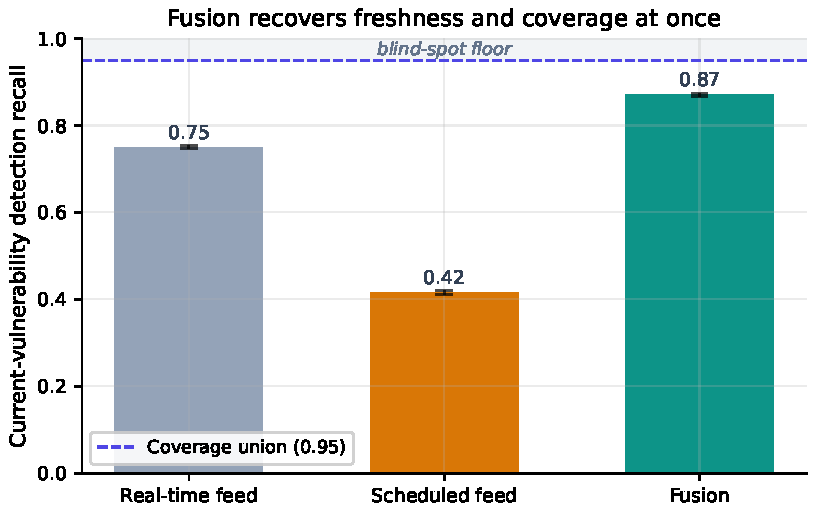
\includegraphics[width=\columnwidth]{fig1_regimes.pdf}
\caption{Detection recall by regime at the reference overlap. Fusion (0.8702) approaches the
coverage union, well above the real-time feed (0.7498) and the scheduled feed; the blind spot is
the floor that fusion cannot cross.\\[2pt]\textit{Alt text:} Bar chart of current-vulnerability detection recall (y-axis 0 to 1) for three regimes on the x-axis: real-time feed at 0.75, scheduled feed at 0.42, and fusion at 0.87, each with a small error bar. A horizontal dashed line at 0.95 marks the coverage union, labelled as the blind-spot floor above the bars.}\label{fig:regimes}\end{figure}

\begin{figure}[t]\centering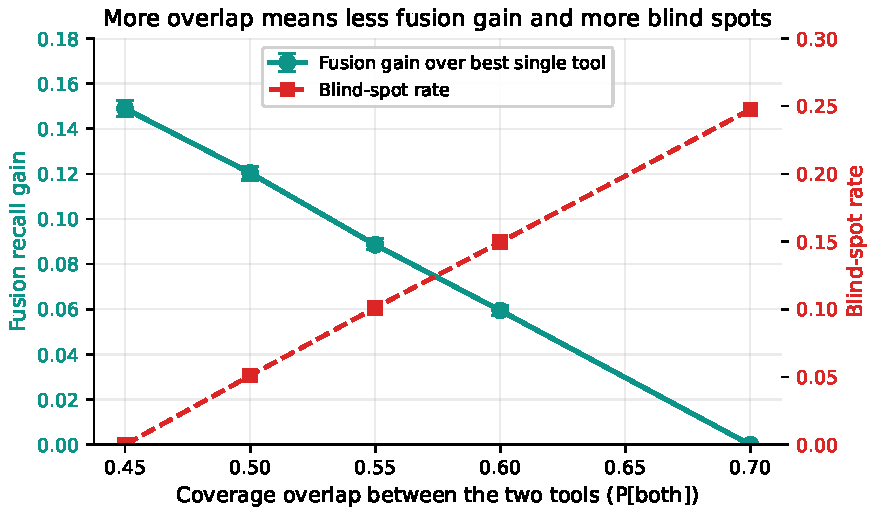
\includegraphics[width=\columnwidth]{fig2_overlap.pdf}
\caption{As coverage overlap rises from 0.45 to 0.70, the fusion gain falls from 0.1489 to 0.0
while the blind spot grows from 0.0 to 0.2475. High overlap removes the gain and enlarges the blind
spot at once.\\[2pt]\textit{Alt text:} Dual-axis line chart with coverage overlap between the two tools on the x-axis (0.45 to 0.70). A solid descending line (left axis, fusion recall gain) falls from about 0.149 to 0.0, while a dashed ascending line (right axis, blind-spot rate) rises from 0.0 to about 0.247; the two lines cross near overlap 0.57.}\label{fig:overlap}\end{figure}

\section{Robustness and Sensitivity}
\label{sec:robustness}
The headline results are reported at the reference overlap, but the contribution of this paper is
structural, and the structure is best seen across the full overlap sweep. This section presents the
complete sweep and then examines the one scenario the model cannot defend against by fusion alone:
an adversary who hides in the blind spot.

\subsection{Full overlap sweep}
Table~\ref{tab:sweep} reports every primary quantity at each of the five overlap levels: the
real-time recall, the scheduled recall, the fused recall, the fusion gain over the better single
feed, and the blind-spot rate, each a mean over the 25 evaluation seeds. The per-feed recalls are
nearly flat across the sweep, near $0.75$ for the real-time feed and near $0.42$ for the scheduled
feed, confirming Eq.~(\ref{eq:single_recalls}): the single-feed recalls depend on coverage and
freshness, not on how the two coverage sets relate. The fused recall, the fusion gain, and the
blind spot, by contrast, all move with the overlap, and they move exactly as the closed-form
analysis of Section~\ref{sec:theory} predicts. The fused recall falls from $0.9001$ at low overlap
to $0.7525$ at full overlap, where it coincides with the real-time recall because the scheduled
feed has no unique fresh asset left to add. The gain falls monotonically from $0.1489$ to $0.0$
while the blind spot grows monotonically from $0.0$ to $0.2475$. The sweep is therefore a
sensitivity analysis on the one parameter that distinguishes a pair of complementary feeds from a
pair of redundant ones, and it shows the gain to be entirely governed by that parameter through
Eq.~(\ref{eq:gain}).

\begin{table}[t]
\centering
\caption{Full overlap sweep: per-feed recall, fused recall, fusion gain over the better single feed,
and blind-spot rate, each a mean over 25 evaluation seeds. Values are read from the frozen primary
results.}
\label{tab:sweep}
\footnotesize
\setlength{\tabcolsep}{4pt}
\begin{tabular}{@{}cccccc@{}}
\toprule
Overlap $p_{\cap}$ & Real-time & Scheduled & Fusion & Gain & Blind-spot $\beta$ \\
\midrule
0.45 & 0.7511 & 0.4194 & 0.9001 & 0.1489 & 0.0000 \\
0.50 & 0.7498 & 0.4153 & 0.8702 & 0.1204 & 0.0510 \\
0.55 & 0.7497 & 0.4200 & 0.8382 & 0.0886 & 0.1012 \\
0.60 & 0.7522 & 0.4213 & 0.8116 & 0.0595 & 0.1495 \\
0.70 & 0.7525 & 0.4210 & 0.7525 & 0.0000 & 0.2475 \\
\bottomrule
\end{tabular}
\end{table}

\subsection{The adversarial blind spot}
The blind-spot floor of Eq.~(\ref{eq:floor}) is a structural limit under benign asset placement, but
it becomes a security property under adversarial placement. Consider an adversary who controls where
a vulnerable asset sits relative to the two feeds' coverage, by introducing an unmanaged host, a
network appliance outside the real-time agent's install base, or a machine the scheduled scanner
never reaches. Such an adversary places the asset in the blind spot, the coverage class that neither
feed sees, of probability $\beta$ in Eq.~(\ref{eq:blindspot}). By the fusion identity
Eq.~(\ref{eq:fuse_recall}), an asset in the blind spot contributes nothing to either term of the
fused recall: the real-time feed does not cover it, so the first term excludes it, and the scheduled
feed does not cover it, so the second term excludes it. The asset is therefore invisible to fusion
\emph{by construction}, not by any failure of the fusion logic, and no decision rule built on these
two feeds can detect it~\cite{cover2006elements}. This is the worst case for a fused heatmap: an
adversary who knows the coverage map can guarantee non-detection by occupying the one region the
union of feeds does not reach. The implication is sharp and matches the deployment guidance:
closing the blind spot requires new coverage, a third feed with complementary reach or the discovery
and onboarding of unmanaged assets, and not a better way of merging the two feeds that already
exist. Refining the fusion rule cannot move an asset out of the blind spot; only extending coverage
can. The blind-spot rate $\beta$ is thus both the benign floor on misses and the adversarial measure
of how much of the fleet an attacker can render invisible by placement alone, and it is the quantity
a visibility program should drive down.

\section{Discussion}
The three findings combine into a single deployment principle: fusion is worth doing exactly to the
extent that the two feeds are complementary, and its value is bounded by what they jointly cover.
The gain is not a property of the fusion algorithm, which is a simple union; it is the
scheduled-only-fresh coverage that the second feed contributes, and the identity in H3 lets a team
estimate it before deploying anything. A team can measure the scheduled feed's coverage outside the
real-time feed's footprint, multiply by its freshness, and read off the gain to within the
resolution of our experiment. Where the two feeds overlap, fusion adds nothing, because the
real-time feed already supplies full freshness there; where neither feed reaches, fusion cannot
help, because the blind spot is a floor that no combination rule can lower.

This reframes the visibility program. The binding constraint on current-vulnerability visibility is
not the sophistication of the fusion, but the blind spot, the assets that neither tool covers. At
the reference overlap that floor is 0.051, and it grows to 0.2475 as the tools become redundant. An
agency that wants to push visibility past the floor must extend coverage, by deploying the
real-time agent more broadly, adding a third feed with complementary reach, or discovering and
onboarding unmanaged assets, rather than refining how the existing two feeds are merged. The
overlap result sharpens the tool-selection decision: agencies should pair tools with complementary
coverage and accept that redundant footprints are doubly wasteful, since they neither add fusion
gain nor shrink the blind spot. The autonomic-computing goal of continuous self-assessment is best
served by feeds chosen for complementarity~\cite{kephart2003vision}.

\subsection{A deployment recipe from the identity}
The closed-form identity turns the design of a fusion deployment into three measurements that a
team can take before committing to any integration work. First, estimate the real-time feed's
coverage and the scheduled feed's coverage independently, for example from each tool's own asset
inventory against the authoritative fleet list. Second, estimate the overlap, the fraction of
assets both feeds reach, since the gain falls as that overlap rises: from 0.1489 at an overlap of
0.45 to 0.0 at an overlap of 0.70, where the second feed is fully redundant. Third, multiply the
scheduled feed's out-of-footprint coverage by its freshness to read off the expected fusion gain
directly, because that product is the scheduled-only-fresh coverage that the identity equates to
the gain. A team that performs these three measurements can predict the value of fusion to within
the resolution of our experiment without integrating anything, and can decline the integration when
the predicted gain is small.

The same measurements bound the residual risk. The blind-spot rate, the fraction of assets neither
feed reaches, is the floor on missed current vulnerabilities and is read off the same coverage
estimates: it is 0.051 at the reference overlap and rises to 0.2475 as the feeds become redundant.
Because that floor is invariant to the fusion rule, it belongs on the visibility program's risk
register as a coverage-extension item, not a fusion-tuning item. The operational ordering follows:
measure coverage and overlap, fuse when the predicted gain justifies the integration, and treat the
blind spot as the next coverage investment. This is the discipline that distinguishes a visibility
program that compounds its feeds from one that merely accumulates redundant ones.

\section{Threats to Validity}
\emph{Construct validity.} The model abstracts detection as a coverage-and-freshness event and a
current vulnerability as a binary per-asset fact. Real feeds report with intermediate confidence,
real coverage is correlated with asset type, and real staleness depends on scan cadence and the
vulnerability change rate. These would shift the absolute recall magnitudes but not the structural
relationships: a blind-spot floor exists whenever any asset is uncovered, the freshness identity
follows from the real-time feed supplying freshness on its own coverage, and the overlap dependence
follows from the coverage accounting of Eq.~(\ref{eq:classes}) and Eq.~(\ref{eq:blindspot}).

\emph{Internal validity.} Because the study is pre-registered and the evaluation seeds 1000 to 1024
were inspected only once, the reported numbers are not the product of analytic search. The model was
developed on separate seeds, and no coverage, overlap, or freshness probability was tuned to clear a
threshold. The evaluation script computes each verdict mechanically from the frozen data.

\emph{External validity.} The fleet size, the coverage marginals, the overlap sweep, and the
freshness probability are documented priors, not measurements from any agency, so absolute recall
values such as 0.8702 should be read as illustrative of the model rather than as field estimates.
The comparative gain, the freshness mechanism, the blind-spot floor, and the overlap dependence
depend on the qualitative structure rather than on the specific constants, and we expect them to
transfer. Calibrating coverage, overlap, and freshness against a real two-tool deployment is the
natural next step.

\emph{Statistical validity.} Intervals are BCa bootstrap intervals over 25 seeds, appropriate for
the small-sample, possibly skewed statistics reported here~\cite{efron1987bca,efron1994introduction};
we use interval non-overlap rather than significance testing throughout, avoiding the
multiple-comparison pitfalls of repeated $p$-values across the hypotheses and overlap levels.

\emph{Scope.} The model omits false positives, which a production heatmap must also manage, and
treats the two feeds' coverage as independent given the overlap parameter. Incorporating a
precision dimension and correlated coverage is left to future work.

\section{Conclusion}
Fusing a fresh-but-partial real-time feed with a broad-but-stale scheduled feed recovers
current-vulnerability visibility that neither achieves alone, but the benefit is governed by the
relationship between the feeds rather than by the fusion logic. In a pre-registered simulation,
fusion raised detection recall from 0.7498 to 0.8702 at the reference overlap, a gain of 0.1204
($[0.1173, 0.1232]$) above a 0.10 bar; that gain equaled exactly the scheduled feed's unique fresh
coverage (difference 0.0); the fusion miss of 0.1298 stayed above a blind-spot floor of 0.051 that
no fusion can cross; and the gain fell monotonically to 0.0 as the feeds became redundant while the
blind spot grew to 0.2475. The deployment guidance is concrete: fuse complementary, low-overlap
feeds, predict the gain from the second feed's unique fresh coverage, and treat the blind spot, not
the fusion logic, as the binding constraint, closing it by extending coverage rather than by
refining the merge. Calibrating the coverage and freshness priors against a real two-tool
deployment is the next step toward turning these structural findings into field estimates.

\section*{Data Availability Statement}
The data and code that support the findings of this study are openly available in the research-papers repository at \url{https://github.com/Harshavardhanmalla-Labs/research-papers/tree/main/paper15}. The manuscript sources, figures, analysis code, and frozen result tables are included and regenerate every reported number deterministically from the fixed seeds.

\section*{Disclosure Statement}
No potential conflict of interest was reported by the author.

\section*{Funding}
No funding was received.

% Generated by IEEEtran.bst, version: 1.14 (2015/08/26)
\begin{thebibliography}{10}
\providecommand{\url}[1]{#1}
\csname url@samestyle\endcsname
\providecommand{\newblock}{\relax}
\providecommand{\bibinfo}[2]{#2}
\providecommand{\BIBentrySTDinterwordspacing}{\spaceskip=0pt\relax}
\providecommand{\BIBentryALTinterwordstretchfactor}{4}
\providecommand{\BIBentryALTinterwordspacing}{\spaceskip=\fontdimen2\font plus
\BIBentryALTinterwordstretchfactor\fontdimen3\font minus
  \fontdimen4\font\relax}
\providecommand{\BIBforeignlanguage}[2]{{%
\expandafter\ifx\csname l@#1\endcsname\relax
\typeout{** WARNING: IEEEtran.bst: No hyphenation pattern has been}%
\typeout{** loaded for the language `#1'. Using the pattern for}%
\typeout{** the default language instead.}%
\else
\language=\csname l@#1\endcsname
\fi
#2}}
\providecommand{\BIBdecl}{\relax}
\BIBdecl

\bibitem{cisabod2301}
{Cybersecurity and Infrastructure Security Agency (CISA)}, ``Binding
  operational directive 23-01: Improving asset visibility and vulnerability
  detection on federal networks,'' U.S. Department of Homeland Security, Tech.
  Rep., Oct. 2022,
  \url{https://www.cisa.gov/news-events/directives/bod-23-01-improving-asset-visibility-and-vulnerability-detection-federal-networks}.

\bibitem{nist80137}
K.~Dempsey, N.~S. Chawla, A.~Johnson, R.~Johnston, A.~C. Jones, A.~Orebaugh,
  M.~Scholl, and K.~Stine, ``Information security continuous monitoring (iscm)
  for federal information systems and organizations,'' National Institute of
  Standards and Technology, Tech. Rep. NIST Special Publication 800-137, 2011.

\bibitem{nist80137a}
K.~Dempsey, V.~Pillitteri, C.~Baer, R.~Niemeyer, R.~Rudman, and S.~Urban,
  ``Assessing information security continuous monitoring (iscm) programs:
  Developing an iscm program assessment,'' National Institute of Standards and
  Technology, Tech. Rep. NIST Special Publication 800-137A, 2020.

\bibitem{hall1997fusion}
D.~L. Hall and J.~Llinas, ``An introduction to multisensor data fusion,''
  \emph{Proceedings of the IEEE}, vol.~85, no.~1, pp. 6-23, 1997.

\bibitem{bass2000fusion}
T.~Bass, ``Intrusion detection systems and multisensor data fusion,''
  \emph{Communications of the ACM}, vol.~43, no.~4, pp. 99-105, 2000.

\bibitem{efron1987bca}
B.~Efron, ``Better bootstrap confidence intervals,'' \emph{Journal of the
  American Statistical Association}, vol.~82, no. 397, pp. 171-185, 1987.

\bibitem{efron1994introduction}
B.~Efron and R.~J. Tibshirani, \emph{An Introduction to the Bootstrap}.\hskip
  1em plus 0.5em minus 0.4em\relax Chapman \& Hall/CRC, 1994.

\bibitem{wohlin2012experimentation}
C.~Wohlin, P.~Runeson, M.~H{\"o}st, M.~C. Ohlsson, B.~Regnell, and
  A.~Wessl{\'e}n, \emph{Experimentation in Software Engineering}.\hskip 1em
  plus 0.5em minus 0.4em\relax Springer, 2012.

\bibitem{chandola2009anomaly}
V.~Chandola, A.~Banerjee, and V.~Kumar, ``Anomaly detection: A survey,''
  \emph{ACM Computing Surveys}, vol.~41, no.~3, pp. 1-58, 2009.

\bibitem{davis2006pr}
J.~Davis and M.~Goadrich, ``The relationship between precision-recall and {ROC}
  curves,'' in \emph{Proceedings of the 23rd International Conference on
  Machine Learning}, 2006, pp. 233-240.

\bibitem{paper4hygieneprio}
H.~Malla, ``{HygienePrio}: Cyber-hygiene signal augmentation for
  {EPSS}-weighted vulnerability prioritization,''
  \url{https://github.com/Harshavardhanmalla-Labs/research-papers/tree/main/paper4},
  2026, companion paper; source, code, and frozen results in the same
  repository.

\bibitem{paper1vulnprio}
H.~Malla, ``Context-aware vulnerability prioritization for government endpoint
  fleets,''
  \url{https://github.com/Harshavardhanmalla-Labs/research-papers/tree/main/paper1},
  2026, companion paper; source, code, and frozen results in the same
  repository.

\bibitem{nist80053}
{Joint Task Force}, ``Security and privacy controls for information systems and
  organizations,'' National Institute of Standards and Technology, Tech. Rep.
  NIST Special Publication 800-53 Rev. 5, 2020.

\bibitem{fips199}
{National Institute of Standards and Technology}, ``Standards for security
  categorization of federal information and information systems,'' U.S.
  Department of Commerce, Tech. Rep. FIPS PUB 199, 2004.

\bibitem{verizon2026dbir}
{Verizon}, ``2026 data breach investigations report ({DBIR}),'' Verizon
  Business, Tech. Rep., 2026,
  \url{https://www.verizon.com/business/resources/reports/dbir/}.

\bibitem{kephart2003vision}
J.~O. Kephart and D.~M. Chess, ``The vision of autonomic computing,''
  \emph{IEEE Computer}, vol.~36, no.~1, pp. 41-50, 2003.

\bibitem{cover2006elements}
T.~M. Cover and J.~A. Thomas, \emph{Elements of Information Theory},
  2nd~ed.\hskip 1em plus 0.5em minus 0.4em\relax Wiley, 2006.

\end{thebibliography}

\end{document}
